% !TeX program = lualatex
% !TeX encoding = utf8
% !TeX spellcheck = uk_UA
% !BIB program = biber

%http://imfn.lviv.ua/zf/?page_id=190

\documentclass{LabBook}
\usetikzlibrary{shapes}
\addbibresource{d:/Projects/LaTeX/MyPackage/MyBase.bib}

\title{Оптика}
\def\subtitle{Лабораторний практикум}
%========================================================================================================
%
% !TeX program = lualatex
% !TeX encoding = utf8
% !TeX spellcheck = uk_UA
% !TeX root =../EMProblems.tex

%========================================================================================================
%
%									      Палітурка
%
%========================================================================================================

% ---------------------------------------- Кольори секцій -----------------------------------------------
\definecolor{themecolordark}{RGB}{34,102,101}
\definecolor{themecolorlight}{RGB}{153,168,167}
\definecolor{titlebgdark}{RGB}{0,103,102}
\definecolor{titlebglight}{RGB}{191,233,251}

\newcommand{\CoverPage}{
	\begin{alwayssingle}
		\begin{center}
			\begin{flushright}\bfseries\sffamily
				\MakeUppercase{Міністерство освіти і науки України}\\
				КПІ ім. Ігоря Сікорського\\
			\end{flushright}
			\begin{tcolorbox}[titlepagestyle,
					toprule=0.10cm,
					bottomrule=0.10cm,
					overlay={%
						\node (picture) at ([xshift=4cm]frame.west) {
\includegraphics{logo_PTI}};
					}
			]%
			\begin{flushright}
				\large\bfseries\color{white}Фізико-технічний інститут
			\end{flushright}
			\end{tcolorbox}

			\vspace*{15em}

			\begin{tcolorbox}[
				titlepagestyle,
				toprule=0.15cm,
				bottomrule=0.15cm,
				top=1.3cm,
				bottom=0.7cm,
				overlay={%
				\node[%
							fill=white,
							rounded corners = 15pt,	
							draw=themecolorlight,
							line width=0.15cm,
							inner sep=0pt,
							text width=17cm,
							minimum height=2cm,
							align=center,
							%anchor=east,
							font=\sffamily\bfseries\large
						] (title) at (frame.north) {С.~М. Пономаренко,
													В.~В. Іванова%
					};
				}
			]
			\centering
			\Huge\sffamily\bfseries\textcolor{white}{\realtitle}\\
			\huge\sffamily\bfseries\textcolor{white}{\subtitle}
			\end{tcolorbox}	
			\vfill
%		 	\begin{Large}\color{themecolordark!90!black}
%			\begin{gather*}
%				\frac{\partial F^{\mu\nu}}{\partial x^\nu} =                                                                                -\frac{4\pi}{c}j^\mu \\
%				\frac{\partial F^{\mu\nu}}{\partial x^\alpha} + \frac{\partial F^{\mu\alpha}}{\partial x^\nu} +\frac{\partial F^{\alpha\mu}}{\partial x^\nu}  = 0.
%			\end{gather*}
%			\end{Large}
			\vfill
			\begin{tcolorbox}[titlepagestyle,
					toprule=0.10cm,
					bottomrule=0.10cm]
				\begin{center}\color{white}\bfseries\normalsize
					\MakeUppercase{Київ~2021} \\
%					КПІ ім. Ігоря Сікорського \\
%					\the\year
				\end{center}			       	
			\end{tcolorbox}
		\end{center}
		\clearpage
	\end{alwayssingle}
\setcounter{page}{1}	
}


%========================================================================================================
%
%									      Титульна сторінка
%
%========================================================================================================

\renewcommand\maketitle{
	\begin{alwayssingle}
		\begin{center}
				\MakeUppercase{Міністерство освіти і науки України}
				
				\bigskip
				\MakeUppercase{Національний технічний університет України}\\
				<<КИЇВСЬКИЙ ПОЛІТЕХНІЧНИЙ ІНСТИТУТ \\ імені ІГОРЯ СІКОРСЬКОГО>>
				\vspace*{150pt}
		
%				{\large С.~Пономаренко,
%						Ю.~О.~Тараненко
%						}
%				\vspace*{50pt}
			
				{\Huge\sffamily\bfseries\realtitle}\\[1em]
				{\huge\sffamily\bfseries\subtitle}	
			
			\vspace*{50pt}
			\begin{center}\itshape
                Рекомендовано Методичною радою КПІ ім. Ігоря Сікорського як навчальний посібник для здобувачів ступеня бакалавра за освітньою програмою <<Прикладна фізика>> спеціальності 105 Прикладна фізика та наноматеріали 
%				Методичні вказівки до виконання лабораторних робіт за темою <<Змінний струм>> з навчальної дисципліни <<Електрика та магнетизм>> для студентів, які навчаються за спеціальністю 105 <<Прикладна фізика та наноматеріали>>
			\end{center}

			\vfill
			\begin{center}
				\MakeUppercase{Київ} \\
				КПІ ім. Ігоря Сікорського \\
				2021
			\end{center}			       	
		\end{center}
		\clearpage
	\end{alwayssingle}	
}


%========================================================================================================
%
%									      Друга сторінка
%
%========================================================================================================
\newcommand\makeinfopage{
	\begin{alwayssingle}
		\noindent%	
        \begin{minipage}[t]{\textwidth}
                \realtitle: \subtitle\ [Електронний ресурс] : навч. посіб. для студ. спеціальностей
                105 <<Прикладна фізика та наноматеріали>> / КПІ ім. Ігоря Сікорського; уклад.  С.~М. Пономаренко, В.~В. Іванова ; КПІ ім. Ігоря Сікорського.~--- Електронні текстові дані
            (1 файл: 0.7~МБ). – Київ : КПІ ім. Ігоря Сікорського, 2021. --- \the\numexpr\getpagerefnumber{LastPage}~с.
        \end{minipage}
        \vspace*{2em}
		\begin{center}\itshape\small
				Гриф надано Методичною радою КПІ ім. Ігоря Сікорського (протокол № 6 від 25.02.2021 р.) за поданням Вченої ради Фізико-технічного інституту (протокол №1 від 11.01.2021 р.)
		\end{center}
		\begin{center}
			Електронне мережне навчальне видання
			%\par {Версія від~\href{http://www.istpravda.com.ua/dates}{\today}} \par\else \par  \fi
		\end{center}
		\begin{center}\bfseries
    		\LARGE\sffamily\realtitle\\
   			\Large\sffamily\subtitle
   		\end{center}

		\vfill\noindent%
        \begin{minipage}[t]{0.2\linewidth}
            	\begin{flushleft}
                    Укладачі:
                \end{flushleft}
        \end{minipage}\hfill
        \begin{minipage}[t]{0.78\linewidth}
		\begin{flushleft}
			\href{http://phes.ipt.kpi.ua/ponomarenko-sergij-mikolajovich}{\itshape Пономаренко Сергій Миколайович}, к.ф.-м.н., доцент \\
			\itshape \href{http://apd.ipt.kpi.ua/kafedra/perspages/IvanovaVV.html}{Іванова Віта Вікторівна}, к.т.н., доцент
		\end{flushleft}
        \end{minipage}

        \vspace*{2em}
		\noindent%
        \begin{minipage}[t]{0.2\linewidth}
            	\begin{flushleft}
                    Відповідальний редактор:
                \end{flushleft}
        \end{minipage}\hfill
        \begin{minipage}[t]{0.78\linewidth}
                к.ф.-м.н., доцент \href{http://ipt.kpi.ua/smirnov}{Смирнов С.~О.}
        \end{minipage}

        \vspace*{2em}
		\noindent%
        \begin{minipage}[t]{0.2\linewidth}
            	\begin{flushleft}
                    Рецензент:
                \end{flushleft}
        \end{minipage}\hfill
        \begin{minipage}[t]{0.78\linewidth}
                \href{http://www.nas.gov.ua/UA/PersonalSite/Pages/default.aspx?PersonID=0000007584}{Лимаренко Руслан Анатолійович}, к.ф.-м.н., с.н.с., учений секретар Міжнародного центру <<Інститут прикладної оптики>>  НАН України
        \end{minipage}

        \vfill

		Розглянуто зміст, основні складові та порядок виконання лабораторних робіт з дисципліни <<Оптика>>. 

		Для студентів фізико-технічного інституту КПІ ім. Ігоря Сікорського, які навчаються за спеціальністю 105~<<Прикладна фізика та наноматеріали>>.
		
		\vfill
				
%		\begin{flushleft}\small
%			Ілюстративний матеріал підручника підготовлений за допомогою пакету \href{http://pgf.sourceforge.net}{TikZ/Pgf}. Верстка тексту проведена в видавничій системі \LaTeXe{} (компілятор Lua\LaTeX) на базі системи комп'ютерної верстки \TeX{} (Збірка  \href{https://www.tug.org/texlive/}{\TeX Live~\the\year}) з використанням оболонки \href{https://www.texstudio.org}{\TeX Studio}.
%		\end{flushleft}	
	\begin{flushright}
        \textcopyright{} С.~М. Пономаренко, В.~В. Іванова, 2021 р.
    \end{flushright}
		\newpage%
	\end{alwayssingle}
}



%					      Титульна сторінка
%
%========================================================================================================
\date{}
\begin{document}
\CoverPage
\maketitle
\makeinfopage
\tableofcontents
\thispagestyle{empty}
\clearpage

%========================================================================================================
%
%									      Вставка файлів розділів
%
%====================================================f====================================================

%\renewcommand{\thechapter}{5.\arabic{chapter}}
\newcommand{\ChaptersInterferention}{
	Lab5_3p1,
	Lab5_3p2,
	Lab5_4,
}
\newcommand{\ChaptersDifraction}{
	Lab5_5,
}
\newcommand{\ChaptersPolarization}{
	Lab5_7,
}
%========================================================================================================
\pagestyle{theorpart}
\renewcommand{\theequation}{\thepart.\arabic{equation}}
\renewcommand{\thefigure}{\thepart.\arabic{figure}}
% !TeX program = lualatex
% !TeX encoding = utf8
% !TeX spellcheck = uk_UA
% !TeX root =../LabWork.tex

\part{Інтерференція світла}

\nocite{akhmanov, Godzhaev}
\printbibliography[title={Рекомендована література}, heading=subbibliography]

\section{Означення}

Під інтерференцією світла розуміють явища, в яких при накладенні двох або більше світлових хвиль відбувається просторовий перерозподіл їх енергії, при цьому виникають стійкі в часі світлі і темні ділянки, що чергуються в просторі --- так звані інтерференційні смуги. 

Нехай в деяку точку приходять дві гармонійні хвилі, напруженості поля яких змінюються згідно із законами:

\begin{equation}\label{eq:EField}
    \vect{E}_1 = \vect{E}_{01}\cos\omega_1 t, \quad \vect{E}_2 = \vect{E}_{02}\cos(\omega_2 t + \phi).
\end{equation}

Відповідно до принципу суперпозиції напруженість результуючої хвилі дорівнює сумі напруженостей вихідних хвиль:

\begin{equation*}
    \vect{E} = \vect{E}_1 + \vect{E}_2,
\end{equation*}

А інтенсивність результуючої хвилі  пропорційна усередненому за часом квадрату напруженості:
\begin{equation}\label{eq:Intens}
    I \sim \left\langle\left(  \vect{E}_1 + \vect{E}_2\right)^2  \right\rangle  = \left\langle E_1^2\right\rangle + \left\langle E_2^2\right\rangle  + 2\left\langle \vect{E}_1 \cdot \vect{E}_2 \right\rangle.
\end{equation}

Доданок $\left\langle \vect{E}_1 \cdot \vect{E}_2 \right\rangle$ називається \emph{інтерференційним}, оскільки саме він відповідальний за існування інтерференційної картини. Цей доданок дорівнює нулю в наступних випадках:
\begin{enumerate}
    \item напрямки коливань векторів $\vect{E}_1 $ та $\vect{E}_2 $ є взаєоперпендмкулярними;
    \item частоти коливань $\omega_1$ та  $\omega_2$ є різними;
    \item різниця фаз хвиль $\phi$ в будь-якій точці простору змінюється дуже швидко (в  порівнянні з часом спостереження) і хаотично.
\end{enumerate}

Отже, для спостереження інтерференційної картини необхідно, щоб всі попередні умови не виконувались.

Розглянемо дві хвилі, які поляризовані в однієї площині, мають однакову частоту і сталу різницю фаз:
\begin{equation}\label{eq:CogEField}
    \vect{E}_1 = \vect{E}_{01}\cos\omega t, \quad \vect{E}_2 = \vect{E}_{02}\cos(\omega t + \phi), \quad \vect{E}_{01} \parallel \vect{E}_{02}.
\end{equation}
такі хвилі називаються \emph{когерентними}. Підставляючи ці вирази в формулу~\eqref{eq:Intens}, знайдемо, що результуюча інтенсивність таких хвиль дорівнюватиме:
\begin{equation}\label{key}
    I = I_1 + I_2 + 2\sqrt{I_1I_2}\cos\phi.
\end{equation}

Крім того, якщо інтенсивності хвиль в певній точці простору однакові $I_1 = I_2 = I_0$, то результуюча інтенсивність дорівнюватиме:
\begin{equation}
    I = 2I_0\left(1+ \cos\phi \right) .
\end{equation}
Отже, як видно з останньої формули, умовою того, що в даній точці буде спостерігатись максимум чи мінімум інтерференційної картини залежить від різниці фаз $\phi$ між хвилями, а саме:
\begin{equation}\label{eq:InterferenceCondition}
    \phi=
    \begin{cases}
        2 m \pi, &\quad \text{умова максимуму інтерференції}, \\
        \left( 2m + 1 \right) \pi , &\quad\text{умова мінімуму інтерференції},
    \end{cases}
\end{equation}
де $m \in \mathbb{Z}$.

\section{Різниця ходу хвиль}

Рівняння гармонічної хвилі має вигляд:
\[
    \vect{E} = \vect{E}_{0}\cos(k r - \omega t),
\]
де аргумент косинуса $ k r - \omega t $,= називається фазою хвилі, а $k = \frac{2\pi}{\lambda}$~--- хвильове число.  Якщо дві монохроматичні хвилі приходять в одну точку простору, то цій точці різниця фаз між хвилями визначається за формулою:
\[
    \phi = ( k_2 r_2 - \omega t) - ( k_1 r_1 - \omega t) = k_2 r_2 - k_1 r_1.
\]

Хвилі можуть поширюватись в різних середовищах з різними показниками заломлення. Хоча хвилі мають однакову частоту, але в середовищах з різним показником заломлення вони мають різну довжину хвилі, яка в $n$ разів ($n$ абсолютний показник заломлення) менша ніж у вакуумі $\lambda = \frac{\lambda_0}{n}$, а тому, хвильове число також буде різним. В оптиці прийнято використовувати саме довжину хвилі світла в вакуумі, а тому різниця фаз буде визначатись як:
\[
    \phi  = k_2 r_2 - k_1 r_1 = \frac{2\pi}{\lambda_0} (n_2 r_2 - n_1 r_1).
\]
Величина 
\begin{equation}\label{eq:optdeiff}
    \Delta = n_2 r_2 - n_1 r_1
\end{equation}
називається оптичною різницею ходу хвиль, натомість величина $r_2 - r_1$ називається геометричною різницею ходу. Не важко зрозуміти, що у вакуумі ці величини співпадають. Крім цього, умови максимуму та мінімуму інтерференції~\eqref{eq:InterferenceCondition} можна переписати для оптичної різниці ходу:
\begin{equation}\label{eq:InterferenceConditionDelta}
    \Delta=
    \begin{cases}
        m \lambda, &\quad \text{умова максимуму інтерференції}, \\
        (2m + 1)\frac{\lambda}{2}, &\quad\text{умова мінімуму інтерференції},
    \end{cases}
\end{equation}
де $m \in \mathbb{Z}$, $\lambda = \frac{\nu}{c}$~--- довжина хвилі світла у вакуумі (індекс <<0>> для зручності не вказаний).

\section{Ітерференційні схеми}

Нехай у нас в розпорядженні є два точкових монохроматичних джерела (довжина хвилі $\lambda$, інтенсивність кожного $I_0$ і розташовані вони на відстані $d$ один від одного. Знайдемо, як буде виглядати інтерференційна картина на екрані віддаленому від джерел на відстань $L \gg d$.

\subsection{Схема Юнга}

Площина екрану паралельна до лінії $\overline{S_1S_2}$, що з'єднує два джерела (рис.~\ref{fig:YoungScheme}). Дане розташування прийнято називати \emph{схемою Юнга}. Знайдемо різницю ходу $\Delta = r_2 - r_1$ між променями, що йдуть від джерел $S_1$ і $S_2$ в точку $P$ з координатою $y$. Початок координат помістимо в точці $O$, відносно якої джерела світла $S_1$ і $S_2$ розташовані симетрично.

\begin{figure}[!h]
	\centering
	\begin{tikzpicture}
		\coordinate (Q) at (0,3.5);
		\coordinate (O1) at (0.25,3.5);
%		\foreach \i in {1,...,3} {\fill[cyan, draw=black] (0,{5/2*(\i-1)}) coordinate (LC\i) rectangle +(0.25,2);}
%		\foreach \i in {0,...,2} {\draw[thick, green!70!blue] (-2-0.5*\i,0) -- +(0,7);}
%		\foreach \i in {0,...,6} {\draw[-latex, orange!80!black] (-3.1,{\i + 0.5}) -- +(1.15,0);}
		\draw[thick] (8,-1) -- coordinate (O) coordinate[pos=0.945] (P) +(0,9); % Ecran
		\fill (P) circle(0.05) node[above left] {$P$};
		\draw (Q) -- (O) node [below left] {$O$};
		\draw[dashed]  (O1) -- (P);
		\draw ([xshift=1.5cm]O1)  let \p{PO1}=( $(P) - (O1)$) in arc (0:atan(\y{PO1}/\x{PO1}):1.5) node[pos=0.5, right] {$\theta$};
		\draw[red!80!black, decoration={
					markings,
					mark=at position 0.5 with {\arrow{latex}}}, postaction={decorate}] (0.25, 2.25 + 2.5) coordinate (S2R) -- node[above, black] {$r_{2}$}(P);
        \fill[red] (S2R) circle(0.1);
		\draw[red!80!black, decoration={
					markings,
					mark=at position 0.5 with {\arrow{latex}}}, postaction={decorate}] (0.25, 2.25 ) coordinate (S1R) -- node[below right, black] {$r_{1}$}  (P);
        \fill[red] (S1R) circle(0.1);
        \draw (S2R) -- (S2R|- 8,-1);
		\draw [dashed] (S2R) -- ($(S1R)!(S2R)!(P)$) coordinate (RA);
		\draw ([yshift=-0.7cm]S2R) let \p{PR}=( $(S2R) - (RA)$) in arc (-90:{atan(\y{PR}/\x{PR})}:0.7) coordinate[pos=0.5] (TH);
		\draw (TH) -- +(60:2) node[above] {$\theta$};
		\draw[decorate,decoration={brace,amplitude=5pt,mirror, raise=0.5ex}] (S1R) -- node[below right=0.5ex] {$\Delta$} (RA);
		\begin{scope}[on background layer]
			\fill[cyan!10] (O1) -- (P) -- (O) -- cycle;
			\fill[yellow!10] (S2R) -- ($(S1R)!(S2R)!(P)$) -- (S1R);
		\end{scope}
		\draw ([xshift=-0.1cm]S2R)  -- coordinate[pos = 0.8] (d2) ([xshift=-1.5cm]S2R) ;
		\draw ([xshift=-0.1cm]S1R)  -- coordinate[pos = 0.8] (d1) ([xshift=-1.5cm]S1R) ;
		\draw (d2) -- node[fill=white] {$d$} (d1);

		\draw ([xshift=0.1cm]P)  -- coordinate[pos = 0.8] (y1) ([xshift=1cm]P) ;
		\draw ([xshift=0.1cm]O)  -- coordinate[pos = 0.8] (y0) ([xshift=1cm]O) ;
		\draw (y1) -- node[fill=white] {$y$} (y0);
		\node at ([shift={(-0.5,0.3)}]S2R) {$S_2$};
		\node at ([shift={(-0.5,-0.3)}]S1R) {$S_1$};

		\draw[latex-latex] (0.25,0.5) -- node[fill=white] {$L$}({P|-0.5,0.5});

		\foreach \i in {-8,...,8} { \path[bottom color=white,  top color=white, middle color = red] (9,{0.5*\i+3.25}) rectangle +(1,0.5); }
	\end{tikzpicture}
	\caption{Схема Юнга}
	\label{fig:YoungScheme}
\end{figure}

Із геометрії рисунка
\begin{align*}
	r_1^2 = {r^2} + {\left( y - \frac{d}{2}\right) ^2}, \\
	r_2^2 = {r^2} + {\left( y + \frac{d}{2}\right) ^2}.
\end{align*}

Звідки випливає, що
\begin{equation*}
	r_2^2 - r_1^2 = 2yd,
\end{equation*}
або
\begin{equation*}
	({r_2} + {r_1})({r_2} - {r_1}) = 2yd.
\end{equation*}

 Відстань $y$, в межах якого утворюються інтерференційні смуги, також значно менше $L$. За цих умова можна вважати, що 
\[{r_2} + {r_1} \cong 2L.\] 

Тоді \[{r_2} - {r_1} = \frac{{yd}}{L}.\] В середовищі з показником заломлення $n \approx 1$ різниця дає оптичну різницю ходу $\Delta$ . Отже, можна написати:
\begin{equation}
	\Delta  = \frac{{yd}}{L}.
\end{equation}

Різниця фаз хвиль $\phi$, яка визначається як:
\begin{equation}\label{eq:Phase_Diff}
    \phi = \frac{2\pi}{\lambda} \Delta
\end{equation}
у випадку схеми Юнга дорівнює:
\[
    \phi = \frac{2\pi}{\lambda} \frac{{yd}}{L}.
\]

Використовуючи умову максимуму інтерференції (для різниці ходу $\Delta = m\lambda$), отримаємо положення самих цих максимумів:
\begin{equation}
	y_{\max} = \frac{{mL}}{d}\lambda.
\end{equation}

Відстань між двома сусідніми максимумами інтенсивності називається відстанню між інтерференційними смугами.  З останнього виразу випливає, що відстань між сусідніми максимумами матиме значення:
\begin{equation}\label{eq:widthofmax}
	\Delta y = \frac{L}{d}\lambda.
\end{equation}

\subsection{Інтерференційні кільця}

Площина екрану перпендикулярна до лінії $\overline{S_1S_2}$, що з'єднує два джерела (рис.~\ref{fig:Rings}). Знову ж знайдемо різницю ходу $\Delta = r_2 - r_1$ між променями, що йдуть від джерел $S_1$ і $S_2$ в точку $P$ з координатою $y$.

\begin{figure}[!h]
	\centering
	\begin{tikzpicture}
		\coordinate (Q) at (0,3.5);
		\coordinate (O1) at (0.25,3.5);
%		\foreach \i in {1,...,3} {\fill[cyan, draw=black] (0,{5/2*(\i-1)}) coordinate (LC\i) rectangle +(0.25,2);}
%		\foreach \i in {0,...,2} {\draw[thick, green!70!blue] (-2-0.5*\i,0) -- +(0,7);}
%		\foreach \i in {0,...,6} {\draw[-latex, orange!80!black] (-3.1,{\i + 0.5}) -- +(1.15,0);}
		\draw[thick] (8,-1) -- coordinate (O) coordinate[pos=0.945] (P) +(0,9); % Ecran
		\fill (P) circle(0.05) node[above left] {$P$};
		\draw (Q) -- (O) node [below left] {$O$};
%		\draw[dashed]  (O1) -- (P);
%		\draw ([xshift=1.5cm]O1)  let \p{PO1}=( $(P) - (O1)$) in arc (0:atan(\y{PO1}/\x{PO1}):1.5) node[pos=0.5, right] {$\theta$};
		\draw[red!80!black, decoration={
					markings,
					mark=at position 0.5 with {\arrow{latex}}}, postaction={decorate}] (0.25, 3.5) coordinate (S2R) -- node[above, black] {$r_{2}$}(P);
        \fill[red] (S2R) circle(0.1);
		\draw[red!80!black, decoration={
					markings,
					mark=at position 0.5 with {\arrow{latex}}}, postaction={decorate}] (2.25, 3.5 ) coordinate (S1R) -- node[below right, black] {$r_{1}$}  (P);
        \fill[red] (S1R) circle(0.1);
        \draw (S2R) -- (S2R|- 8,-1);
%		\draw [dashed] (S2R) -- ($(S1R)!(S2R)!(P)$) coordinate (RA);
		\draw ([xshift=0.7cm]S2R) let \p{PR}=( $(S2R) - (P)$) in arc (0:{atan(\y{PR}/\x{PR})}:0.7) node[anchor = west, pos=0.7] {$\theta$};

		\draw ([xshift=0.7cm]S1R) let \p{PR}=( $(S1R) - (P)$) in arc (0:{atan(\y{PR}/\x{PR})}:0.7) node[anchor = west, pos=0.7] {$\theta$};

		\draw[decorate,decoration={brace,amplitude=5pt, raise=0.5ex}] (S2R) -- node[pos=0.5, above=1ex] {$\Delta$} ($(S2R)!(S1R)!(P)$);

		\draw (S1R) -- ($(S2R)!(S1R)!(P)$);

		\draw ([yshift=-0.1cm]S2R)  -- coordinate[pos = 0.8] (d2) ([yshift=-1.5cm]S2R) ;
		\draw ([yshift=-0.1cm]S1R)  -- coordinate[pos = 0.8] (d1) ([yshift=-1.5cm]S1R) ;
		\draw[latex-latex] (d2) -- node[fill=white] {$d$} (d1);

		\draw ([xshift=0.1cm]P)  -- coordinate[pos = 0.8] (y1) ([xshift=1cm]P) ;
		\draw ([xshift=0.1cm]O)  -- coordinate[pos = 0.8] (y0) ([xshift=1cm]O) ;
		\draw (y1) -- node[fill=white] {$y$} (y0);
		\node at ([shift={(-0.5,-0.3)}]S2R) {$S_2$};
		\node at ([shift={(-0.5,-0.3)}]S1R) {$S_1$};

		\draw[latex-latex] (0.25,0.5) -- node[fill=white] {$L$}({P|-0.5,0.5});
        \foreach \i in {1,...,10} {\draw[red, line width = {10- \i}] ($(y0)-(-3.5,0)$) circle ({sqrt(\i)});}
%		\foreach \i in {-8,...,8} { \path[bottom color=white,  top color=white, middle color = red] (9,{0.5*\i+3.25}) rectangle +(1,0.5); }
	\end{tikzpicture}
	\caption{Схема для спостереження інтерференційних кілець}
	\label{fig:Rings}
\end{figure}

Оскільки така схема симетрична щодо повороту навколо лінії $\overline{S_1S_2}$, то інтерференційна картина на екрані буде являти собою систему концентричних кіл (інтерференційних кілець).

Різниця ходу хвиль, як не важко розрахувати, використовуючи розкладання косинуса в ряд, дорівнюватиме:
\begin{equation}\label{key}
    \Delta \approx d\left( 1 - \frac{\theta^2}{2}\right) \approx d\left( 1 - \frac{y^2}{2L^2}\right).
\end{equation}

Максимальний порядок інтерференції буде в центрі картини і дорівнює:
\[
    m_{\max} = \frac{d}{\lambda}
\]
і по мірі віддалення від центру порядок інтерференції зменшується. 

Оскільки $m_{\max}$ може приймати довільні значення, то в центрі може
спостерігатися як темна, так і світла пляма. Знайдемо вираз для радіусів
кілець. Нехай, наприклад, в центрі картини темна пляма, тобто:
\[
    d = \left( m_0 + \frac12 \right)\lambda = \Delta_0, 
\]
де $m \in \mathbb{Z}$.  Для $k$-го темного кільця ($k = 1,2,3,\ldots$) різниця ходу дорівнюватиме:
\[
    \Delta_i = \Delta_0 - k\lambda = d\left( 1 - \frac{y_k}{2L^2}\right),
\]
звідки
\begin{equation}\label{eq:RingRadius}
    y_k^2 = \frac{2\lambda L^2}{d} k.
\end{equation}

Цей вираз дозволяє знайти радіуси кілець $y_k$, порядок інтерференції яких дорівнює $m_{\max} - k$.

\subsection{Довільне розташування екрану відносно джерел}

У загальному випадку при довільному розташуванні екрана відносно точкових монохроматичних джерел інтерференційна картина буде являти собою систему дуг кіл (рис. \ref{fig:IntPic}).

\begin{figure}
\centering
  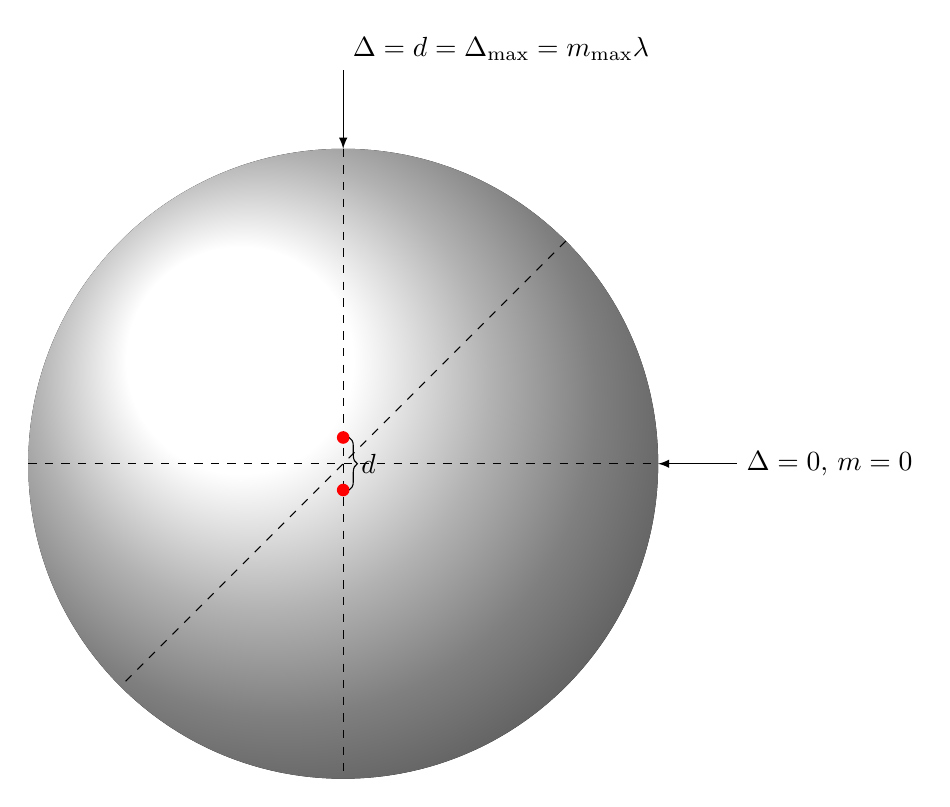
\begin{tikzpicture}
  \def\R{4} % sphere radius
  \def\Elevation{20} % elevation angle
 

  \fill[ball color=white!10] (0,0) circle (\R); % 3D lighting effect

\foreach \i in {89,86,...,59} {
\DrawLatitudeCircle{\i}
\DrawLatitudeCircle{-\i}
}
\foreach \i in {-6,-3,...,6} {\DrawLatitudeCircle{\i}}
\draw[dashed] (0,\R) -- (0,-\R);
\draw[dashed] (-\R,0) --(\R,0);
\draw[dashed] (45:\R) -- (225:\R);
\fill[red] (0,\R/12) coordinate (S1) circle (0.08);
\fill[red] (0,-\R/12) coordinate (S2) circle (0.08);
		\draw[decorate,decoration={brace,amplitude=3pt, raise=0.5ex}] (S1) -- node[right=3pt] {$d$} (S2);

\draw[latex-] (90:\R) -- ++(90:1) node[above right] {$\Delta = d= \Delta_{\max} = m_{\max}\lambda$};
\draw[latex-] (0:\R) -- ++(0:1) node[right] {$\Delta = 0$, $m = 0$};
\end{tikzpicture}  
\caption{Інтерференційні картини при різних положеннях екрану
відносно двох точкових монохроматичності джерел}
\label{fig:IntPic}
\end{figure}

\section{Реальні схеми спостерження інтерференції}

Для отримання когерентних світлових хвиль застосовують спеціальні експериментальні методи. Ці методи можна розділити на два класи:
\begin{itemize}
	\item методи поділу хвильового фронту;
	\item методи поділу амплітуди.
\end{itemize}

Їх ідея полягає в тому, щоб використовувати випромінювання одних і тих самих атомів джерела.

В \emph{методі поділу хвильового фронту} інтерферують хвилі, що йдуть від різних ділянок хвильового фронту. На цьому методі побудовано класичні інтерференційні схеми: дзеркало Ллойда, біпрізма Френеля, білінзи, бідзеркала, дослід Юнга тощо \cite[\S  5, стор. 81]{Godzhaev}.

В \emph{методі поділу амплітуди} пучок ділиться на одній або декількох пропускаючих поверхнях, що частково відбивають світло. Амплітуда кожної з інтерферуючих хвиль меньша ніж амплітуда вихідної хвилі. Даний метод використовується для спостереження інтерференційної картини в тонких плівках, інтерферометрі Майкельсона, інтерферометрі Фабрі-Перо \cite[\S 6, стор. 85]{Godzhaev}.

Якщо джерело світла точкове, то в результаті застосування оптичної схеми будь-якого з методів розподілу (хвильового фронту або амплітуди) виникнуть два точкових зображення джерела, які стануть новими когерентними джерелами. Випромінювання від цих нових джерел буде поширюватися, взагалі кажучи, не у всіх напрямках (це залежить від
оптичної схеми). Інтерференція буде спостерігатися в області накладення
світлових пучків від обох джерел (в області інтерференції) при будь-якому
розташуванні екрана. У цьому випадку говорять, що інтерференційна картина
не локалізована. Як вже зазначалося вище, вигляд інтерференційної картини
залежить від взаємного розташування лінії, що з'єднує джерела, і
площині екрану. Якщо лінія паралельна площині екрану (схема Юнга), то
спостерігаються смуги. Якщо лінія перпендикулярна площині екрану, то
спостерігається система кілець.
\renewcommand{\theequation}{\thechapter.\arabic{equation}}
\renewcommand{\thefigure}{\thechapter.\arabic{figure}}
\labworklayout
\pagestyle{main}
\multiinclude{\ChaptersInterferention}[]
%========================================================================================================
\pagestyle{theorpart}
\setcounter{section}{0}
\setcounter{equation}{0}
\setcounter{figure}{0}
\renewcommand{\theequation}{\thepart.\arabic{equation}}
\renewcommand{\thefigure}{\thepart.\arabic{figure}}
% !TeX program = lualatex
% !TeX encoding = utf8
% !TeX spellcheck = uk_UA
% !TeX root =../LabWork.tex

\part{Дифракція світла}

\nocite{akhmanov, Godzhaev}
\printbibliography[title={Рекомендована література}, heading=subbibliography]

\section{Означення}

Дифракція світла --- це сукупність фізичних явищ, обумовлених хвильовою природою світла і спостерігаються при його поширенні в середовищі з різко вираженою оптичної неоднорідністю (наприклад, при проходженні через отвори в екранах, поблизу меж непрозорих тіл тощо). У більш вузькому сенсі під дифракцією розуміють огинання світлом різних перешкод, тобто відхилення від законів геометричної оптики. Точна теорія дифракції навіть для простих випадків є собою досить складною в математичному відношенні. Серед багатьох методів наближеного розв'язання задачі історично першим, найбільш простим і наочним, був метод, який в даний час прийнято називати \emph{принципом Гюйгенса-Френеля}. Гюйгенс, вперше обґрунтував хвильову теорію світла, запропонував наступну побудова: кожна точка довільного хвильового фронту стає джерелом елементарних сферичних вторинних хвиль, при цьому хвильовий фронт в будь-який інший момент є огинаючою цих вторинних хвиль. Френель доповнив принцип Гюйгенса твердженням про когерентність джерел вторинних хвиль, що дозволило йому розглядати основні дифракційні явища як результат інтерференції вторинних хвиль. Це поєднання побудови Гюйгенса з принципом інтерференції Френеля отримало назва \emph{принципу Гюйгенса-Френеля}, який, хоча і є наближеним, дозволяє кількісно описати дифракційні явища, які спостерігаються на простих об'єктах.

Математичне обгрунтування принципу Гюйгенса-Френеля було в подальшому дано Кірхгофом, який, зокрема, показав, що в якості поверхні вторинних джерел може бути вибрана не тільки поверхня хвильового фронту, але і будь-яка замкнута поверхня, всередині якої знаходиться точка спостереження. Пояснимо далі ідею Кірхгофа.

\begin{wrapfigure}{O}{0.45\linewidth}
	\centering
	\begin{tikzpicture}
		\draw[fill=gray!50] (-0.9,-1.9) -- (-0.9,1.9) -- (0.9,2.5) -- (0.9,-1.2) -- cycle;
		\draw[fill=white] (0.02,0.3) ellipse (0.6 and 1.5) ;
        \node at (0,0) {$\Sigma$};
        \draw[*-latex, dash pattern=on 1.34cm off 0.49cm] (-2,0)  node[left] {$S_0$} -- node[pos=0.3,above] {$r$} ++(35:2.5) coordinate (A);
        \draw[dashed] (A) -- ++(35:2) coordinate[pos=0.5] (A1);
        \draw[-latex] (A) --  node[above] {$s$} (4,0) coordinate (P) node[right] {$P$};
        \draw (A1) arc(35:-20:1) node[pos=0.5,right] {$\alpha$};
	\end{tikzpicture}
	\caption{Ілюстрація}
	\label{pic:Diffraction}
\end{wrapfigure}
Нехай на шляху сферичної монохроматичної світлової хвилі, що виходить із точкового джерела $S_0$, знаходиться плоский непрозорий об'єкт з отвором $\Sigma$, розміри якого великі в порівнянні з довжиною хвилі (рис.~\ref{pic:Diffraction}). Відповідно до принципу Гюйгенса-Френеля напруженість поля в точці $P$ за об'єктом визначається суперпозицією хвиль від вторинних джерел, розташованих в площині отвору $\Sigma$. При цьому амплітуда і фаза вторинних
сферичних хвиль, що приходять в точку $P$, залежать як від відстані $r$ (від джерела $S_0$ до відповідних ділянок хвильового фронту, що лежить на поверхні $\Sigma$), так і від відстані $s$ (від цих ділянок до точки $P$).

У загальному випадку комплексна амплітуда поля $E_P$ може бути знайдена з
допомогою інтегральної формули Френеля-Кірхгофа:

\begin{equation}\label{eq:Fr-Kirch}
    E_P = \iint\limits_{\Sigma}  \frac{A e^{ikr}}{r}K(\alpha) \frac{e^{iks}}{s} dS,
\end{equation}
де $k = \frac{2\pi}{\lambda}$~--- хвильове число, $\alpha$~--- кут між напрямками $r$ та $s$, $K(\alpha)$~--- фактор Френеля, що описує залежність амплітуди вторинних хвиль від кута $\alpha$ між напрямками поширення падаючої і вторинної хвилі, $dS$~--- елемент площі в площині отвору $\Sigma$,  $A$~--- константа. Інтегрування ведеться по <<відкритій>> в об'єкті поверхні $\Sigma$.

У цій формулі множник $\frac{e^{ikr}}{r}$ описує сферичну хвилю, що поширюється від точки $S_0$ до довільного вторинного джерела, розташованого на поверхні $\Sigma$, множник $\frac{e^{iks}}{s}$~--- сферичну хвилю, що йде від вторинного джерела до точки спостереження $P$.

Найбільш цікавим для розгляду є випадок, коли характерний лінійний розмір отвору малий у порівнянні з відстанями $r$ і $s$ від точок $S_0$ і $P$ до об'єкта. У цьому випадку як фактор $K(\alpha)$, так і множник $\frac{1}{rs}$ незначно змінюються при інтегруванні по отвору $\Sigma$ і основну роль в обчисленні дифракційної картини за формулою~\eqref{eq:Fr-Kirch} відіграє інтеграл від швидко множника вигляду $e^{ik(r+s)}$, який швидко осцилює. Розкладання в ряд цього множника дозволяє істотно спростити формулу~\eqref{eq:Fr-Kirch}. Явища, які описуються в рамках такого наближення, носять назва дифракції Френеля, або дифракції в ближній зоні. При $r \to \infty$ фронт падаючої хвилі можна вважати плоским. Якщо $s \to \infty$, то і вторинні хвилі, поширюються під деяким кутом $\alpha$ до початкового напрямку, утворюють плоский хвильовий фронт. Дифракційні явища, які спостерігаються при цих умовах, носять назву дифракції Фраунгофера, або дифракції в далекій зоні. Кількісний критерій, що дозволяє розрізняти наближення Френеля і Фраунгофера, буде наведено нижче після введення поняття зон Френеля.

\begin{figure}[h!]
	\centering
\begin{tikzpicture}[rotate=-90]
    \def\R{4} % sphere radius
    \def\Elevation{25} % elevation angle
    \fill[ball color=white!10] (0,0) circle (\R); % 3D lighting effect
    \foreach \i in {30,40,...,89} {\DrawLatitudeCircle[black]{\i}}
    \draw (0,\R) -- node[below] {$b$} (0,12) coordinate (P) node[below] {$P$};
    \draw (0,0) node[below] {$S_0$} -- node[below] {$a$} (0,\R);
    \NewLatitudePlane[Frensel]{\R}{15}{-180-30};
    \path[Frensel] (0:\R) coordinate (Pprime);
    \draw[] (0,0) ++(0,0.5)arc (90:{180-30}:0.5) node[pos=0.3, anchor = south west] {$\theta$};
    \draw (0,0) -- node[pos=0.6,anchor = east] {$a$} (Pprime);
    \draw (Pprime) -- node [above, sloped, rotate=-90] {$s=b+m\frac\lambda2$} (P);
    \fill[red] (0,0) circle (0.08);
    \fill[red] (P) circle (0.08);
\end{tikzpicture} 
	\caption{Ілюстрація методу зон Френеля}
	\label{pic:Diffraction2}
\end{figure}

Розглянемо надалі круглий отвір на який падає сферичний фронт хвилі. Оскільки інтегрування буде вестись по поверхні фронту, що увійшов в отвір, то $r = a$ змінюватись при інтегруванні не буде. Крім того, елемент поверхні фронту матиме вигляд:
\[
    dS = 2\pi a^2 \sin\theta d\theta = 2\pi \frac{a}{a + b} s ds
\]
 а тому, інтеграл~\eqref{eq:Fr-Kirch} матиме вигляд:
\begin{equation}\label{eq:Fr-KirchSpher}
    E_P =  \frac{2\pi Ae^{ika}}{a + b} \int K(\alpha) e^{iks} ds.
\end{equation}

Точне обчислення інтегралу~\eqref{eq:Fr-KirchSpher}, звичайно, неможливо без знання виду функції $K(\alpha)$. Однак Френель, використовуючи той факт, що довжини світлової хвилі, дуже мала, дав метод наближеного обчислення подібних інтегралів, який називається \emph{методом зон Френеля}. Розіб'ємо сферичний фронт на кільцеві області таким чином, щоб відстань від границь цих областей до точки спостереження дорівнювала $b$, $b + \frac\lambda2$, \ldots,  $b + m\frac\lambda2$, \ldots  (рис.~\ref{pic:Diffraction2}). Ці кільцеві області називаються \emph{зонами Френеля}. Зважаючи на малість довжини хвилі, функція $K(\alpha)$ в межах однієї зони може вважатися постійною. У цьому наближенні інтеграл~\eqref{eq:Fr-KirchSpher} по $m$-й зоні буде дорівнювати:
\begin{equation}\label{eq:Fr-KirchSpher_m}
    E_m = \frac{2\pi Ae^{ika}}{a + b} \cdot K_m\int\limits_{r + (m-1)\frac\lambda2}^{r + m\frac\lambda2}   e^{iks} ds = \frac{2\pi Ae^{ika}}{a + b} \cdot (-1)^{m+1}K_m \frac{e^{ikb}}{ik},
\end{equation}
де $K_m$~--- фактор Френеля для $m$-ї зони.

Результат дії усіх зон в точці $P$ є сумою амплітуд усіх зон:
\begin{equation}\label{eq:SumAmpl}
    E_p = \sum\limits_{m} E_m =\frac{2\pi \frac{A}{a+b}e^{ik(a + b)}}{ik}  \sum\limits_{m} (-1)^{m+1}K_m
\end{equation}

Те, що знаки сусідніх  доданків в сумі~\eqref{eq:SumAmpl} протилежні, означає, що коливання, що вносяться сусідніми зонами Френеля, протилежні по фазі, це слід було очікувати, оскільки вже із самої побудови зон Френеля видно, що  коливання  сусідніх зон запізнюються одне відносно одного на половину довжини хвилі.

Отже, якщо на шляху хвильового фронту поставити перешкоду у вигляді отвору, наприклад, який відкриває $N$ зон Френеля, то неважко показати, що результуюча амплітуда в точці $P$ буде дорівнювати:
\begin{equation}
    E = 
    \begin{cases}
        E_1 + |E_N|, \quad N = 2m \\
        E_1 - |E_N|, \quad N = 2m+1,
    \end{cases}
\end{equation}
Тобто, якщо отвір відкриває парне число зон $N = 2m$, то в точці $P$ спостерігатиметься максимум (світда пляма), а якщо отвір відкриває непарне число зон  $N = 2m + 1$ , то в точці $P$ спостерігатиметься мінімум (темна пляма), а навколо цієї точки чергуватимуться темні та світлі кільця. Однак, оскільки $|E_1|>|E_2|> \ldots >|E_N|$, то у випадку, якщо отвір відкриває багато зон Френеля $N \gg 1$, то $|E_1| \gg |E_N| $, тому амплітуда $E \approx \frac12 E_1$, що означатиме що в центрі буде завжди світла пляма.

Таким чином за умов дифракції на круглому отворі діаметру $D$ від точкового джерела, інтенсивіність світла обумовлюється кількістю відкритих зон $N$ пов'язаних таким співвідношенням:
\begin{equation}\label{eq:Zone_Diameter}
    \frac{D}{2}=r_{m}=\sqrt{m\lambda\frac{ab}{a+b}},
\end{equation}
де $r_{m}$~--- радіус $m$-ї зони Френеля. 

 Оскільки сумарна амплітуда~\eqref{eq:SumAmpl} є знакозмінним рядом, то закривши парні, або непарні зони, можна значно підвищити амплітуду в точці $P$. Для цього треба виготовити екран, який для деяких конкретних значень $a$ та $b$ відкривав би тільки парні або непарні зони. Тоді хвилі від відкритих зон надходили б у точку $Р$ синфазно і інтерференційно підсилювали одну одну. Такий екран називають \emph{зонною платівкою Френеля}. Переписавши формулу \eqref{eq:Zone_Diameter} в вигляді
\begin{equation}\label{eq:Focuse}
    \frac1b+\frac1a=\frac{m\lambda}{r_{m}^{2}}
\end{equation}
    отримаємо формулу для радіусів кілець зонної платівки Френеля. Порівнявши \eqref{eq:Focuse} з формолою тонкої лінзи $\frac1b + \frac1a  = \frac1f$, можна зробити висновок, що зонна платівка працює як лінза з фокусною відстанню
\begin{equation}
    f=\frac{r^{2}_{m}}{m\lambda}.
\end{equation}

Для того, щоб визначити характер дифракції користуються критерієм. Оскільки, вигляд дифракційної  картини залежить від того скільки відкрито зон Френеля, то для визначення умов дифракції зручно ввести параметр, який є числом відкритих зон
\begin{eqnarray}
    m =\frac1D{\sqrt{\lambda\frac{ab}{a + b}}}
\end{eqnarray}
    де $D$~--- характерні розміри отвору.  За умови $m\gg1$ дифракційні ефекти незначні, і розподіл інтенсивності можна описати на основі  геометричної оптики. Для $m\approx1$, отвір або екран перекривають декілька зон Френеля, і має місце дифракція Френеля. Для $m\ll1$ відкрита лише незначна частина першої зони Френеля~--- можна вважати хвильовий фронт плоским, тобто має місце дифракція в  паралельних променях, або \emph{дифракція Фраунгофера}.



\renewcommand{\theequation}{\thechapter.\arabic{equation}}
\renewcommand{\thefigure}{\thechapter.\arabic{figure}}
\labworklayout
\pagestyle{main}
\multiinclude{Lab5_5}[]
%========================================================================================================
\pagestyle{theorpart}
\setcounter{section}{0}
\setcounter{equation}{0}
\setcounter{figure}{0}
\renewcommand{\theequation}{\thepart.\arabic{equation}}
\renewcommand{\thefigure}{\thepart.\arabic{figure}}
\renewcommand{\theequation}{\thepart.\arabic{equation}}
% !TeX program = lualatex
% !TeX encoding = utf8
% !TeX spellcheck = uk_UA
% !TeX root =../LabWork.tex

\part{Поляризація світла}

\nocite{akhmanov, Godzhaev}
\printbibliography[title={Рекомендована література}, heading=subbibliography]

\section{Означення}

Світлові хвилі є електромагнітними, тому вони поперечні. Наприклад, радіохвилі, що випромінюються штирьовою антеною у хвильовій зоні мають вигляд, зображений на рис~\ref{fig:linearPolarisation}. 

\begin{figure}[!h]\centering
% Electromagnetic wave - colored
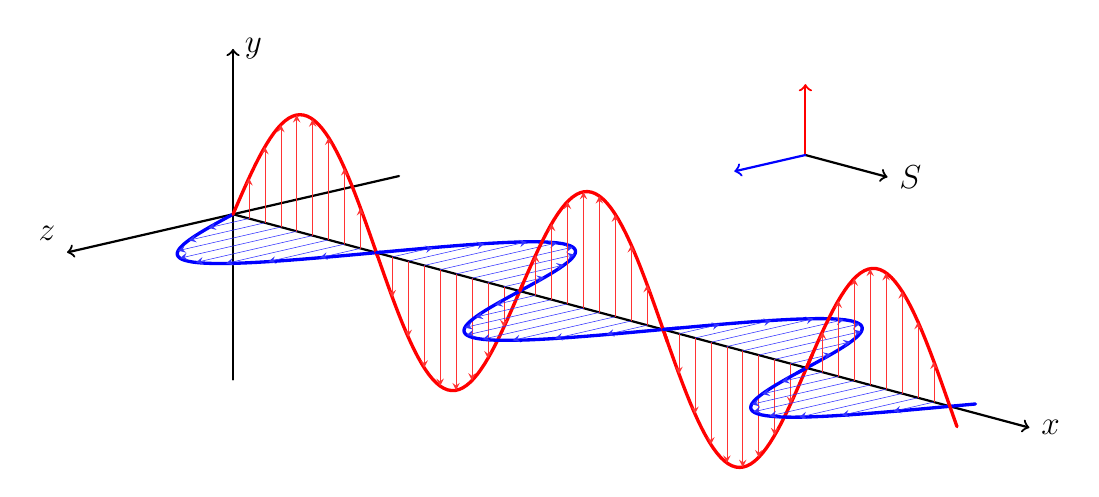
\begin{tikzpicture}[x=(-15:1.2), y=(90:1.0), z=(-150:1.0),
                    line cap=round, line join=round,
                    axis/.style={black, thick,->},
                    vector/.style={>=stealth,->}]
  \large
  \def\A{1.5}
  \def\nNodes{5} % use even number
  \def\nVectorsPerNode{8}
  \def\N{\nNodes*40}
  \def\xmax{\nNodes*pi/2*1.01}
  \pgfmathsetmacro\nVectors{(\nVectorsPerNode+1)*\nNodes}
 
 
  \def\drawENode{ % draw E node and vectors with some offset
    \draw[red,very thick,variable=\t,domain=\iOffset*pi/2:(\iOffset+1)*pi/2*1.01,samples=40]
      plot (\t,{\A*sin(\t*360/pi)},0);
    \foreach \k [evaluate={\t=\k*pi/2/(\nVectorsPerNode+1);
                           \angle=\k*90/(\nVectorsPerNode+1);}]
                in {1,...,\nVectorsPerNode}{
      \draw[vector, help lines, red!80]  (\iOffset*pi/2+\t,0,0) -- ++(0,{\A*sin(2*\angle+\iOffset*180)},0);
    }
  }
  \def\drawBNode{ % draw B node and vectors with some offset
    \draw[blue,very thick,variable=\t,domain=\iOffset*pi/2:(\iOffset+1)*pi/2*1.01,samples=40]
      plot (\t,0,{\A*sin(\t*360/pi)});
    \foreach \k [evaluate={\t=\k*pi/2/(\nVectorsPerNode+1);
                           \angle=\k*90/(\nVectorsPerNode+1);}]
                in {1,...,\nVectorsPerNode}{
      \draw[vector,help lines, blue!80]  (\iOffset*pi/2+\t,0,0) -- ++(0,0,{\A*sin(2*\angle+\iOffset*180)});
    }
  }
 
  % main axes
  \draw[axis] (0,0,0) -- ++(\xmax*1.1,0,0) node[right] {$x$};
  \draw[axis] (0,-\A*1.4,0) -- (0,\A*1.4,0) node[right] {$y$};
  \draw[axis] (0,0,-\A*1.4) -- (0,0,\A*1.4) node[above left] {$z$};
 
  % small axes
  \def\xOffset{{(\nNodes-2)*pi/2}}
  \def\yOffset{\A*1.2}
  \def\zOffset{\A*1.2}
  \draw[axis,black] (\xOffset,\yOffset,-\zOffset) -- ++(\A*0.6,0,0) node[right,align=center] {$\vect{S}$}; %\\propagation
  \draw[axis,red]  (\xOffset,\yOffset,-\zOffset) -- ++(0,\A*0.6,0) node[right] {$\Efield$};
  \draw[axis,blue]   (\xOffset,\yOffset,-\zOffset) -- ++(0,0,\A*0.6) node[above left] {$\Bfield$};
 
  % equation

 
  % draw (anti-)nodes
  \foreach \iNode [evaluate={\iOffset=\iNode-1;}] in {1,...,\nNodes}{
    \ifodd\iNode \drawBNode \drawENode % E overlaps B
    \else        \drawENode \drawBNode % B overlaps E
    \fi
  }
 
\end{tikzpicture}
%  \begin{tikzpicture}[x={(-10:1cm)},y={(90:1cm)},z={(210:1cm)},>={stealth}]
%    % Axes
%    \draw (-1,0,0) node[above] {$x$} -- (5,0,0);
%    \draw[-latex] (0,0,0) -- (0,2,0) node[above] {$y$};
%    \draw[-latex] (0,0,0) -- (0,0,2) node[left] {$z$};
%    % Propagation
%    \draw[->,ultra thick] (5,0,0) -- node[above] {$c$} (6,0,0);
%    % Waves
%    \draw[thick, red] plot[domain=0:4.5,samples=200] (\x,{cos(deg(pi*\x))},0);
%    \draw[gray,thick,blue] plot[domain=0:4.5,samples=200] (\x,0,{cos(deg(pi*\x))});
%    % Arrows
%    \foreach \x in {0.1,0.3,...,4.4} {
%      \draw[->,help lines, red] (\x,0,0) -- (\x,{cos(deg(pi*\x))},0);
%      \draw[->,help lines, blue] (\x,0,0) -- (\x,0,{cos(deg(pi*\x))});
%    }
%    % Labels
%    \node[above right] at (0,1,0) {$\Efield$};
%    \node[below] at (0,0,1) {$\Bfield$};
%  \end{tikzpicture}
\caption{Лінійно поляризоване світло}
\label{fig:linearPolarisation}
\end{figure}

При розгляді таких явищ, як поляризація світла, зазвичай всі міркування пов'язують з площиною коливань вектора напруженості електричного поля $\Efield$~--- світлового вектора, так як хімічний, фізіологічний та інші види впливу світла на речовину обумовлені головним чином електричними коливаннями. Однак при цьому слід пам'ятати про обов'язкове існування перпендикулярного йому вектора напруженості магнітного поля $\Bfield$.

На відміну від електромагнітної хвилі, що випромінюється антеною, світло випромінюється тілами і складається з хвиль, які випускають його окремі атоми. Випромінювання окремого атома триває близько $10^{-8}$~с і являє собою, як кажуть, цуг хвиль довжиною в середньому близько $3$~м. Випромінюючи, атом через деякий час, прийшовши в збуджений стан, випромінює знову і так повторюється знову. Одночасно випромінює безліч атомів. Породжені ними цуги хвиль, накладаючись один на одного, утворюють світлову хвилю. Напрями коливань для кожного цуга орієнтовані випадковим чином. Тому в результуючій світловій хвилі коливання світлового вектора відбуваються в різних напрямках з однаковою ймовірністю. Це треба розуміти так, що при проходженні світлової хвилі через деяку точку коливання світлового вектора швидко і безладно змінюють один одного. Але в межах деякого короткого часу ми маємо справу зі світловим вектором, напрямок коливань якого зберігається, потім напрямок коливань змінюється на інший і т. д. 



При це модуль світлового вектора залишається незмінним.  Таке світло називають \emph{природним}. Умовно це зображують як на рис.~\ref{fig:NonPolarisation}. Світло, в якому напрям коливань світлового вектора упорядкований якимось чином, називають поляризованим. Якщо коливання світлового вектора відбуваються тільки в одній площині, світло називають плоско (або лінійно) поляризованим, так, як це показано на рис.~\ref{fig:linearPolarisation}. Якщо кінець світлового вектора описує еліпс, то такий світло називають еліптично-поляризованим (зокрема, поляризованим по колу, рис.~\ref{fig:CircularPolarisation}).



\begin{figure}[!h]\centering
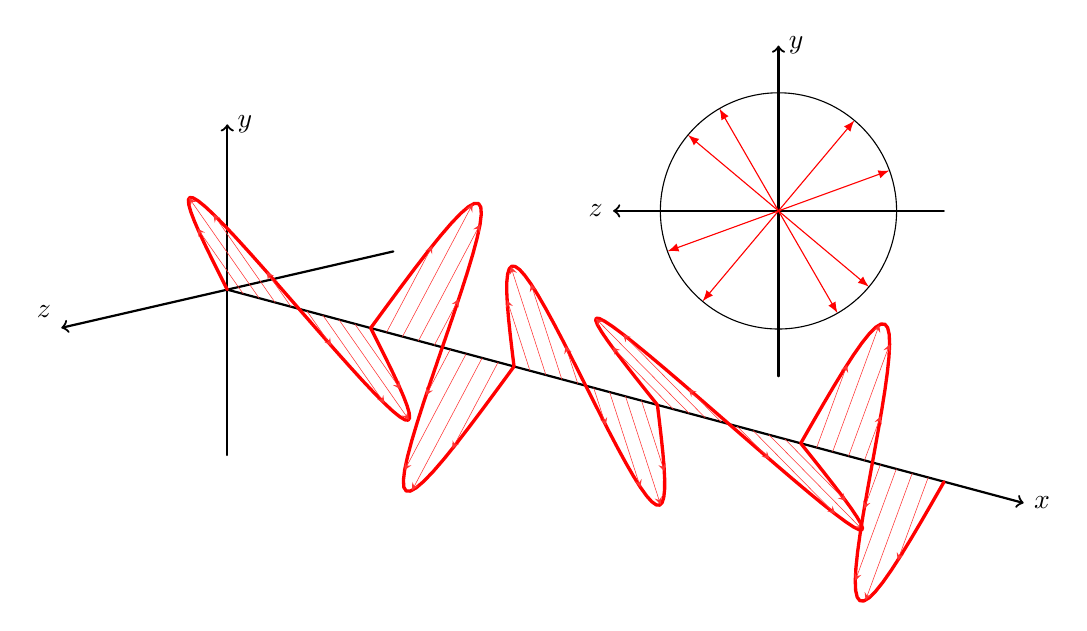
\begin{tikzpicture}[coord/.style={x=(-15:1.2), y=(90:1.0), z=(-150:1.0)},
                    line cap=round, line join=round,
                    axis/.style={black, thick,->},
                    vector/.style={>=stealth,->}]
%  \large
  \def\A{1.5}
  \def\nNodes{5} % use even number
  \def\nVectorsPerNode{8}
  \def\N{\nNodes*40}
  \def\xmax{\nNodes*pi/2*1.01}
  \pgfmathsetmacro\nVectors{(\nVectorsPerNode+1)*\nNodes}
 
 
  \def\drawENode#1{ % draw E node and vectors with some offset
    \draw[coord, red,very thick,variable=\t,domain=\iOffset*pi/2:(\iOffset+1)*pi/2*1,samples=40]
      plot (\t,{\A*sin(4*deg(\t))},{#1*\A*sin(4*deg(\t))});
  \foreach \k [evaluate={\t=\k*pi/2/(\nVectorsPerNode+1);
                           \angle=\k*90/(\nVectorsPerNode+1);}]
                in {1,...,\nVectorsPerNode}{
      \draw[coord, vector, help lines, red!80]  (\iOffset*pi/2+\t,0,0) -- ++(0,{\A*sin(4*deg(\t))},{#1*\A*sin(4*deg(\t))});
    }
  }

 
  % main axes
  \draw[axis, coord] (0,0,0) -- ++(\xmax*1.1,0,0) node[right] {$x$};
  \draw[axis, coord] (0,-\A*1.4,0) -- (0,\A*1.4,0) node[right] {$y$};
  \draw[axis, coord] (0,0,-\A*1.4) -- (0,0,\A*1.4) node[above left] {$z$};
 
  % small axes
  \def\xOffset{{(\nNodes-2)*pi/2}}
  \def\yOffset{\A}
  \def\zOffset{\A}
   \coordinate (O) at (7,1); 
%  \draw[axis,black] (\xOffset,\yOffset,-\zOffset) -- ++(\A*0.6,0,0) node[right,align=center] {$e$}; 
    \draw[axis]  (O) -- +(-90:\A*1.4) -- +(90:\A*1.4) node[right] {$y$};
    \draw[axis]  (O) --  +(0:\A*1.4) -- +(180:\A*1.4) node[left] {$z$};

  \draw[-latex,red]  (O) -- +(-60:\A);
  \draw[-latex,red]  (O) -- +(120:\A);

  \draw[-latex,red]  (O) -- +(-130:\A);
  \draw[-latex,red]  (O) -- +(50:\A);

  \draw[-latex,red]  (O) -- +(-40:\A);
  \draw[-latex,red]  (O) -- +(140:\A);

  \draw[-latex,red]  (O) -- +(-160:\A);
  \draw[-latex,red]  (O) -- +(20:\A);

%     \draw[axis,red]  (7,2) -- ++(180-120:\A);
  \draw[black]  (O) circle (\A);

 
  % draw (anti-)nodes
\def\iOffset{0} \drawENode{0.6}
\def\iOffset{1} \drawENode{-0.6}
\def\iOffset{2} \drawENode{0.3}
\def\iOffset{3} \drawENode{0.8}
\def\iOffset{4} \drawENode{-0.4}
\end{tikzpicture}
\caption{Неполяризоване (природне) світло}
\label{fig:NonPolarisation}
\end{figure}



\begin{figure}[!h]\centering
% Electromagnetic wave - circular polarization
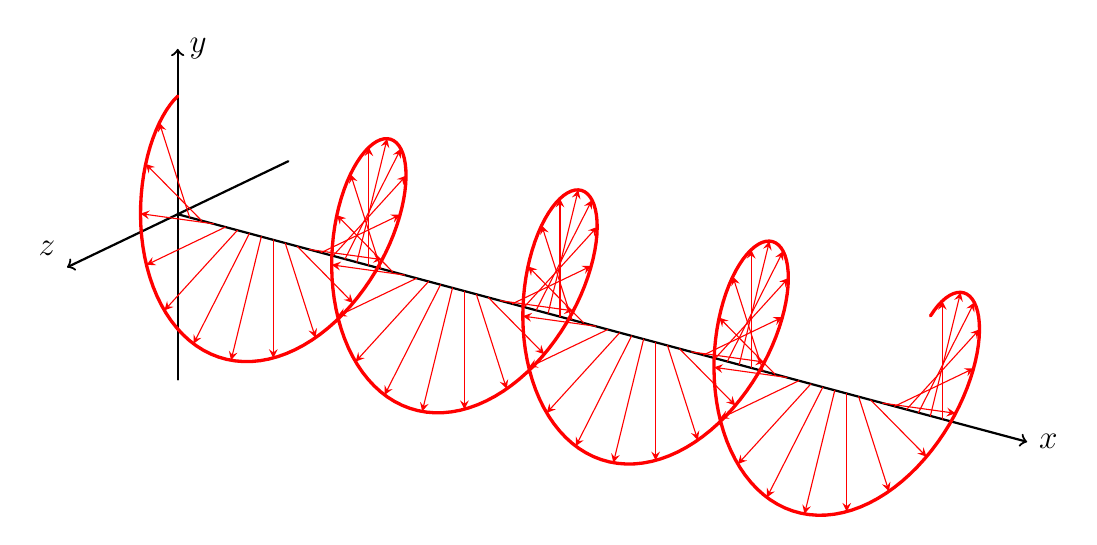
\begin{tikzpicture}[x=(-15:0.8), y=(90:1.0), z=(-150:1.0),
                    line cap=round, line join=round,
                    axis/.style={black, thick,->},
                    vector/.style={>=stealth,->}]
  \large
  \def\A{1.5}
  \def\nNodes{8} % use even number
  \def\nVectorsPerNode{8}
  \def\N{\nNodes*40}
  \def\xmax{\nNodes*pi/2*1.01}
  \pgfmathsetmacro\nVectors{\nVectorsPerNode*\nNodes}
 
 
  % main axes
  \draw[axis] (0,0,0) -- ++(\xmax*1.1,0,0) node[right] {$x$};
  \draw[axis] (0,-\A*1.4,0) -- (0,\A*1.4,0) node[right] {$y$};
  \draw[axis] (0,0,-\A*1.4) -- (0,0,\A*1.4) node[above left] {$z$};
 
  % waves
  \draw[red,very thick,variable=\t,domain=0:\nNodes*pi/2*1.01,samples=\N]
    plot (\t,{\A*cos(\t*360/pi)},{\A*sin(\t*360/pi)});
 
  % draw vectors
  \foreach \k [evaluate={\t=\k*pi/2/\nVectorsPerNode;
                         \angle=\k*90/\nVectorsPerNode;}]
              in {1,...,\nVectors}{
    \draw[vector, red] (\t,0,0) -- ++(0,{\A*cos(2*\angle)},{\A*sin(2*\angle)});
  }
 
\end{tikzpicture}
\caption{Світло, поляризоване по колу}
\label{fig:CircularPolarisation}
\end{figure}

З природного світла можна отримати плоскополяризоване за допомогою приладів, які називаються поляризаторами. Ці прилади вільно пропускають коливання світлового вектора, паралельні площині, яку ми будемо називати площиною пропускання поляризатора. Коливання ж, перпендикулярні до цієї площини, затримуються повністю або частково. У першому випадку поляризатор є ідеальним.

Крім плоскополяризованого і природного світла існує ще <<проміжний>> випадок ---
це частково-поляризоване світло. Частково-поляризоване світло, як і природне, можна представити у вигляді накладення
двох некогерентних плоскополяризованих хвиль з взаємно перпендикулярними площинами поляризації, але різними за інтенсивністю. Його також можна розглядати як суміш природною  і плоскополяризованого складових.

Частково-поляризоване світло характеризують ступенем поляризації $P$, яку визначають як:
\begin{equation}\label{eq: PolarizationLevel}
    P = \frac{I_{\max} - I_{\min}}{I_{\max} + I_{\min}} = \frac{I_\text{пол}}{I_0},
\end{equation}
де $I_0 = I_{\max} + I_{\min}$~--- інтенсивність падаючого на аналізатор світла, $I_\text{пол}$~--- інтенсивність поляризованої компоненти світла. 

Для плоскополяризованого світла $I_\text{пол} = I_0$, а тому ступінь поляризації $P = 1$, для природного світла $I_\text{пол} = 0$, тому  $P = 0$. Це два крайніх випадки. Однак,  що для еліптично-поляризованого світла поняття <<ступінь поляризації>> не застосовне, а тому і формула~\eqref{eq: PolarizationLevel} також не застосовна.

\subsection{Закон Малюса}

Поляризатори можна використовувати і в якості аналізаторів~--- для визначення характеру і ступеня поляризації світла.
Нехай на аналізатор падає лінійно-поляризоване світло, вектор $\Efield$ якого становить кут $\phi$ з площиною пропускання
поляризатора. Аналізатор пропускає тільки ту складову вектора $\Efield$, яка паралельна площині пропускання, тобто $\Efield_0 \cos\phi$ (рис.~\ref{label}). Інтенсивність пропорційна квадрату модуля світлового вектора, тому інтенсивність світла, яке пройшло аналізатор визначається за формулою:
\begin{equation}\label{eq:MaluseLow}
    I = I_0\cos^2\phi.
\end{equation}

\begin{figure}[!h]\centering
\colorlet{crystal}{blue!75}
\begin{tikzpicture}[coord/.style={x=(-15:1.2), y=(90:1.0), z=(-150:1.0)},
                    line cap=round, line join=round,
                    axis/.style={black, thick,->},
                    vector/.style={>=stealth,->},
                    plate/.style={coord, fill, opacity=0.875},]
%  \large
  \def\A{1.5}
  \def\nNodes{5} % use even number
  \def\nVectorsPerNode{8}
  \def\N{\nNodes*40}
  \def\xmax{\nNodes*pi/2*1.01}
  \pgfmathsetmacro\nVectors{(\nVectorsPerNode+1)*\nNodes}
 
 
  \def\drawENode#1#2{ % draw E node and vectors with some offset
    \draw[coord, red,very thick,variable=\t,domain=\iOffset*pi/2:(\iOffset+1)*pi/2,samples=40]
      plot (\t,{\A*#2*sin(4*deg(\t))},{#1*#2*\A*sin(4*deg(\t))});
  \foreach \k [evaluate={\t=\k*pi/2/(\nVectorsPerNode+1);
                           \angle=\k*90/(\nVectorsPerNode+1);}]
                in {1,...,\nVectorsPerNode}{
      \draw[coord, vector, help lines, red!80]  (\iOffset*pi/2+\t,0,0) -- ++(0,{\A*#2*sin(4*deg(\t))},{#1*#2*\A*sin(4*deg(\t))});
    }
  }

 
  % main axes
  \draw[axis, coord] (0,0,0) -- ++(\xmax*1.3,0,0) node[right] {$x$};
  \draw[axis, coord] (0,-\A*1.4,0) -- (0,\A*1.4,0) node[right] {$y$};
  \draw[axis, coord] (0,0,-\A*1.4) -- (0,0,\A*1.4) node[above left] {$z$};
 
  % small axes


 
  % draw (anti-)nodes
\def\iOffset{0} \drawENode{0.6}{1}
\def\iOffset{1} \drawENode{-0.6}{1}
\begin{scope}[xscale=2, yscale=2]
    \def\XOffset{1*pi/2}
    \path [crystal!25, plate] 
        (\XOffset,-1,-1) -- (\XOffset,-1,1) -- (\XOffset,1,1) -- (\XOffset,1,-1) -- cycle;
    \path [crystal!50, plate] 
        (\XOffset,-1,1) -- ({\XOffset-0.1},-1,1) -- ({\XOffset-0.1},1,1) -- (\XOffset,1, 1) -- 
        cycle;
    \path [crystal!75, plate] 
        (\XOffset,1,-1) -- ({\XOffset-0.1},1,-1) -- ({\XOffset-0.1},1,1) -- (\XOffset,1, 1) -- cycle;
    \draw[-latex, plate] (\XOffset,-1,0) -- (\XOffset,1,0) ;
    \draw[-latex, plate] (\XOffset,0,-1) -- (\XOffset,0,1) ;
%    \node [yslant=tan(\xangle), text=crystal!50, below, font=\small] at 
%        (-1,-1,0){Linear Polarizer};
\end{scope}
\def\iOffset{2} \drawENode{0}{0.6}
\def\iOffset{3} \drawENode{0}{0.6}

\begin{scope}[xscale=2, yscale=2]
    \def\XOffset{2*pi/2}
    \path [crystal!25, plate, rotate around={25:(\XOffset,0,0)}] (\XOffset,-1,-1) -- (\XOffset,-1,1) -- (\XOffset,1,1) -- (\XOffset,1,-1) -- cycle;
    \path [crystal!50, plate,rotate around={25:(\XOffset,0,0)}] 
        (\XOffset,-1,1) -- ({\XOffset-0.1},-1,1) -- ({\XOffset-0.1},1,1) -- (\XOffset,1, 1) -- 
        cycle;
    \path [crystal!75, plate, rotate around={25:(\XOffset,0,0)}] 
        (\XOffset,1,-1) -- ({\XOffset-0.1},1,-1) -- ({\XOffset-0.1},1,1) -- (\XOffset,1, 1) -- cycle;
    \draw[-latex, plate,dashed] (\XOffset,-1,0) -- (\XOffset,1,0) coordinate[pos=0.75] (A1);
    \draw[-latex, plate,dashed] (\XOffset,0,-1) -- (\XOffset,0,1) ;

    \draw[-latex, plate,rotate around={25:(\XOffset,0,0)}] (\XOffset,-1,0) -- (\XOffset,1,0) coordinate[pos=0.75] (A2) ;
    \draw[-latex, plate, rotate around={25:(\XOffset,0,0)}] (\XOffset,0,-1) -- (\XOffset,0,1) ;
    
    \draw[->] (A1) to[bend right] node[above] {$\phi$} (A2);

    \node [coord, yslant=tan(15), text=crystal!50, below, font=\small] at 
        (0.1,-1,0) {Не поляризоване світло};
    \node [coord, yslant=tan(15), text=crystal!50, below, font=\small] at 
        (2,-1,1.5) {Поляризоване, $I_0$};
    \node [coord, yslant=tan(15), text=crystal!50, below, font=\small] at 
        (4,-1,1.5) {Поляризоване, $I = I_0\cos^2\phi$};
\end{scope}
\def\iOffset{4} \drawENode{0.5}{0.4}
\def\iOffset{5} \drawENode{0.5}{0.4}
\end{tikzpicture}
\label{fig:MaluseLaw}
\caption{Проходження світла через систему <<поляризатор-аналізатор>>.}
\end{figure}

\subsection{Поляризація при відбиванні та заломленні світла. Кут Брюстера}

Якщо кут падіння природного світла на межу розділу двох прозорих діелектриків відмінний від нуля, то відбитий і заломлений пучки виявляються частково-поляризованими. У відбитому світлі переважають коливання вектора $\Efield$, перпендикулярні до площини падіння, а в переломленому світлі~--- паралельні площині падіння. Ступінь поляризації обох хвиль (відбитої і заломленої) залежить від кута падіння. При деякому значенні кута падіння відбите світло стає повністю поляризованим, і його площина поляризації (площина коливань вектора $\Efield$) виявляється перпендикулярною до площини падіння. Цей кут задовольняє наступній умові:
\begin{equation}\label{eq:BrusterLaw}
    \tg i_\text{Б} = \frac{n_2}{n_1}
\end{equation}

\begin{figure}[!h]\centering
\begin{tikzpicture}
\def\dotMarkRightAngle[size=#1](#2,#3,#4){%
 \draw ($(#3)!#1!(#2)$) -- 
       ($($(#3)!#1!(#2)$)!#1!90:(#2)$) --
       ($(#3)!#1!(#4)$);
}
        \coordinate (O) at (0,0);
%    	\draw (-3,-3) to [grid with coordinates] (3,3);
        \fill[cyan!50] (-3,-3) rectangle (3,0);
        \draw (0,-1) -- (0,1);
        \draw[latex-] (0,0) -- (90+55:3);
        \foreach \i in {0.1,0.2,...,0.9} {\draw[-latex] (0,0) -- (90-55:3) node[fill, circle ,draw=black,scale=0.25, pos=\i]  {} coordinate[pos=0.05] (A1);}
        \foreach \i in {0.1,0.3,...,0.8} {\draw[-latex] (0,0) -- (-90+35:3) node[fill, circle ,draw=black,scale=0.25, pos=\i]  {} 
        node[rotate=-8, draw, strike out, scale=0.9, pos=\i+0.05]  {} 
        node[rotate=-8, draw, strike out, scale=0.9, pos=\i+0.1]  {} 
        node[rotate=-8, draw, strike out, scale=0.9, pos=\i+0.15]  {}
        node[fill, circle ,draw=black,scale=0.25, pos=0.9]  {}  
        coordinate[pos=0.05] (A2) ;}
        \draw[stealth-] (0,0) ++(0,0.5)  arc(90:{90+55}:0.5)  node[pos=0.5, above] {$i_\text{Б}$} ;
        \dotMarkRightAngle[size=6pt](A1,O,A2);
        \node at (2.5,-0.5) {$n_2$};
        \node at (2.5,+0.5) {$n_1$};
	\end{tikzpicture}
\label{fig:Intermedia}
\caption{Падіння світла на границю розділу двох діелектриків}
\end{figure}

Можна переконатися, що при падінні світла під кутом Брюстера відбитий і заломлений промені взаємно ортогональні. При падінні природного світла під кутом Брюстера на межу розділу двох прозорих діелектриків заломлена хвиля стає частково-поляризованою, причому ступінь поляризації її виявляється максимальною.

Закон Брюстера є наслідком формул Френеля, які дають змогу розрахувати інтенсивності відбитого світла від межі розділу:
\begin{align}
    I_{\perp}^{\prime} &= I_{\perp}\frac{\sin^2(i - r)}{\sin^2(i + r)}, \\
    I_{\parallel}^{\prime} &= I_{\parallel}\frac{\tg^2(i - r)}{\tg^2(i + r)}, \label{eq:FrenselParallel}
\end{align}
де $i$~--- кут падіння, $r$~--- кут відбивання, $I_{\perp}$, $I_{\parallel}$~--- інтенсивності падаючого світла, $I_{\perp}^{\prime}$, $I_{\parallel}^{\prime}$~--- інтенсивності відбитого світла, індекси $\perp$ та $\parallel$ відповідають поляризації, перпендикулярній ($s$-поляризація) і паралельній ($p$-поляризація) площині падіння, відповідно.

\renewcommand{\theequation}{\thechapter.\arabic{equation}}
\renewcommand{\thefigure}{\thechapter.\arabic{figure}}
\labworklayout
\multiinclude{\ChaptersPolarization}[]

\end{document}
